\documentclass[10pt, a4paper]{article}
\usepackage[paper=a4paper, left=1.5cm, right=1.5cm, bottom=1.5cm, top=3.5cm]{geometry}
%\usepackage[latin1]{inputenc}
\usepackage[T1]{fontenc}
\usepackage[spanish]{babel}
\usepackage{indentfirst}
\usepackage{fancyhdr}
\usepackage{latexsym}
\usepackage{amsmath}
\usepackage{lastpage}
\usepackage{framed}
\usepackage{todonotes} % para dejar notitas de to-do!
\usepackage{util/aed2-symb,util/aed2-itef,util/aed2-tad,util/aed2-diseno}
\usepackage[colorlinks=true, linkcolor=blue]{hyperref}
\usepackage{setspace}
\usepackage{calc}
\usepackage{hyperref}
\usepackage{xcolor}
\usepackage[table]{xcolor}
\usepackage{verbatim}
\usepackage{tikz}
\usepackage{listingsutf8}
\renewcommand{\lstlistingname}{Código}% Listing -> Código
\definecolor{light-gray}{gray}{0.95}
\lstdefinestyle{styleMatriz}{
    keywords={Para, Función, Devolver, Si, Terminar},
    basicstyle=\tt,
    keywordstyle=\color{blue}, % Color azul para palabras clave
    commentstyle=\color{gray},
    stringstyle=\color{red!70!black},
    frame=single,
    backgroundcolor=\color{light-gray},
    escapeinside={(*}{*)},
    numbers=left,
    numberstyle=\tiny,
    numbersep=10pt,
    literate={:=}{{\ensuremath{\gets}}}1
    {:and}{{\ensuremath{\land}}}1
    {:or}{{\ensuremath{\lor}}}1
    {:distinto}{{\ensuremath{\neq}}}1
    {á}{{\'a}}1 {é}{{\'e}}1 {ó}{{\'o}}1 {í}{{\'i}}1  {ú}{{\'u}}1 
}
\patchcmd{\thebibliography}{\section*{\refname}}{}{}{}
\usepackage{graphicx,subcaption} % Required for inserting images
\usepackage{caption}
\graphicspath{ {img/} }
\usepackage{util/caratula}
\usepackage{minted}

%

% ========== Para escribir pseudo ==========
\usepackage{algorithm}
\usepackage[noend]{algpseudocode}  % "noend" es para no mostrar los endfor, endif
\algrenewcommand\alglinenumber[1]{\tiny #1:}  % Para que los numeros de linea del pseudo sean pequeños
\renewcommand{\thealgorithm}{}  % Que no aparezca el numero luego de "Algorithm"
\floatname{algorithm}{}    % Entre {  } que quiero que aparezca en vez de "Algorithm"
\newcommand{\asignar}[2]{#1 $\gets$ #2}
% traducciones
\algrenewcommand\algorithmicwhile{\textbf{while}}
\algrenewcommand\algorithmicdo{\textbf{do}}
\algrenewcommand\algorithmicreturn{\textbf{return}}
\algrenewcommand\algorithmicif{\textbf{if}}
\algrenewcommand\algorithmicthen{\textbf{then}}
\algrenewcommand\algorithmicfor{\textbf{for}}
%=========================================================


%comandos para cross validation
\newcommand*\revealcline{\noalign{\vskip\arrayrulewidth}}
\newcommand*\nextrow[1]
  {\\\cline{#1}\noalign{\vskip1ex}\cline{#1}\revealcline}
\newcount\ccellA
\newcommand*\ccell[2]
  {%
    \def\tmpa{}%
    \ccellA=1
    \loop
      \ifnum#1=\ccellA
        \edef\tmpa{\unexpanded\expandafter{\tmpa\cellcolor{ccellcolor}}}%
      \fi
    \ifnum#2>\ccellA
      \advance\ccellA1
      \edef\tmpa{\unexpanded\expandafter{\tmpa&}}%
    \repeat
    \tmpa
  }
\usetikzlibrary{matrix}


\newcommand{\f}[1]{\text{#1}}
\renewcommand{\paratodo}[2]{$\forall~#2$: #1}
\newcommand{\numeroEjercicio}[1]{\textbf{\large{Ejercicio #1:}}\\}
\newcommand{\tituloSubEjercicio}[1]{$\newline$\tadNombre{#1:}}

\sloppy

\hypersetup{%
 % Para que el PDF se abra a página completa.
 pdfstartview= {FitH \hypercalcbp{\paperheight-\topmargin-1in-\headheight}},
 pdfauthor={DC - UBA},
 pdfkeywords={Informe Aprendizaje Automático Clasificador Genomas ARN},
 pdfsubject={Informe Aprendizaje Automático}
}

\parskip=5pt % 10pt es el tamaño de fuente

% Pongo en 0 la distancia extra entre ítemes.
\let\olditemize\itemize
\def\itemize{\olditemize\itemsep=0pt}

% Acomodo fancyhdr.
\pagestyle{fancy}
\thispagestyle{fancy}
\addtolength{\headheight}{1pt}
\lhead{Aprendizaje Automático}
\rhead{$1^{\mathrm{er}}$ cuatrimestre de 2025}
\cfoot{\thepage /\pageref{LastPage}}
\renewcommand{\footrulewidth}{0.4pt}

\author{Aprendizaje Automático, DC, UBA.}
\date{}
\title{Informe de trabajo Pr\'actico de Aprendizaje Automático}

\NeedsTeXFormat{LaTeX2e}


% ----- Algunas variables --------------------------------------------------

\let\Materia\relax
\let\Submateria\relax
\let\Titulo\relax
\let\Subtitulo\relax
\let\Grupo\relax

% Comandos para cositas de complejidad

\newcommand{\bigO}{\mathcal{O}} 
\newcommand{\Nat}{\mathbb{N}}
\newcommand{\R}{\mathbb{R}}
\newcommand{\Rpos}{\mathbb{R}_{>0}}
\newcommand{\eqdef}{\overset{\mathrm{def}}{=}}
\newcommand{\eqprop}{\overset{\mathrm{prop}}{=}}
%\newcommand{\ssi}{\leftrightarrow}

\renewcommand{\labelitemi}{$\bullet$} 

\begin{document}

\titulo{Trabajo Práctico}
\subtitulo{Clasificación de expresiones genómicas.}
\fecha{\today}
\materia{Aprendizaje Automático}
\grupo{Trabajo grupal}

\integrante{Braginski Maguitman, Leonel Alan}{385/21}{leobraginski@gmail.com}
\integrante{Moraut, Tobias}{1507/21}{tobiasmoraut7@gmail.com}
\integrante{Bramati, Bianca}{1893/21}{biancabramati2@gmail.com}
\integrante{Care, Damian}{875/02}{damianos.care@gmail.com}
\integrante{??, Leon}{??/??}{??}

\maketitle

\section*{Abstract}
En este trabajo, nos ocuparemos de la realización de un clasificador de genomas mediante aprendizaje automático.
Contamos con un dataset de mediciones de ARN de 200 genes, estas mediciones son información recopilada proveniente de células de pacientes con lesiones pre-tumorales, nuestro objetivo es armar un modelo que logre predecir si las células evolucionarán a un tumor maligno.
Contamos con 500 muestras de mediciones, donde cada muestra está etiquetada por buen o mal pronostico.
A partir de toda esta información, usando distintos algoritmos de aprendizaje automático y explorando todo el espacio del problema, buscamos dar con un modelo final que haya aprendido a clasificar estos pronósticos sobre nuevas muestras nunca antes vistas.

\section*{Separación de datos}
Antes de comenzar a entrenar el modelo, es indispensable separar los datos en conjuntos de entrenamiento y evaluación.
Al finalizar el entrenamiento, estimaremos la performance de nuestro modelo con los datos de evaluación, para lograr estimar un resultado  lo mas cercano a la realidad posible.

Nuestra decisión fue separar un 15\% de los datos para evaluación y el sobrante 85\% para entrenamiento.
Como queremos que nuestro modelo sea entrenado y validado con las mismas frecuencias en clases,
nos encargamos de que la separación mantenga la misma proporción de clases, además de realizar un \textit{shuffle} de los datos previo a la separación.


\begin{figure}[H]
    \centering
    \subfloat[\centering Dataset completo \label{fig:classDistrCompl}]{
        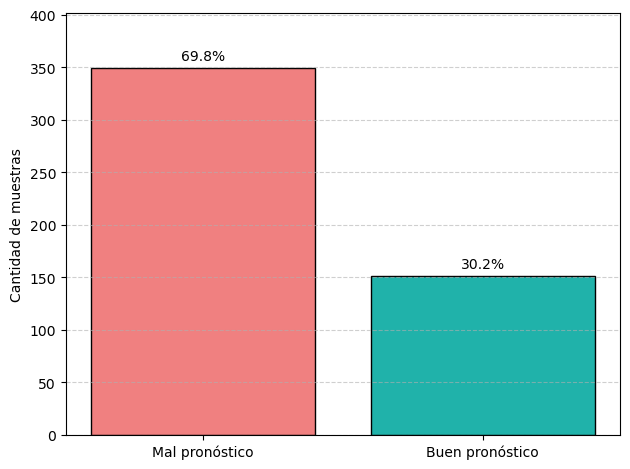
\includegraphics[width=0.25\linewidth]{img/class_distr_compl.png}
    }
    \hspace{0.05\linewidth}
    \subfloat[\centering Datos de entrenamiento \label{fig:distr1}]{
        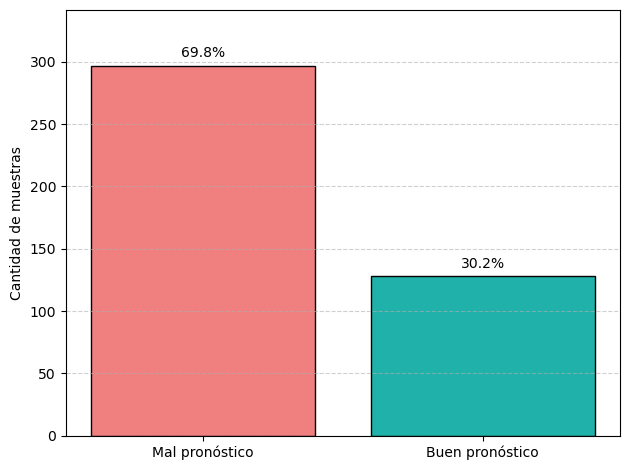
\includegraphics[width=0.25\linewidth]{img/class_distr_train.png}
    }
    \hspace{0.05\linewidth}
    \subfloat[\centering Datos de evaluación \label{fig:distr2}]{
        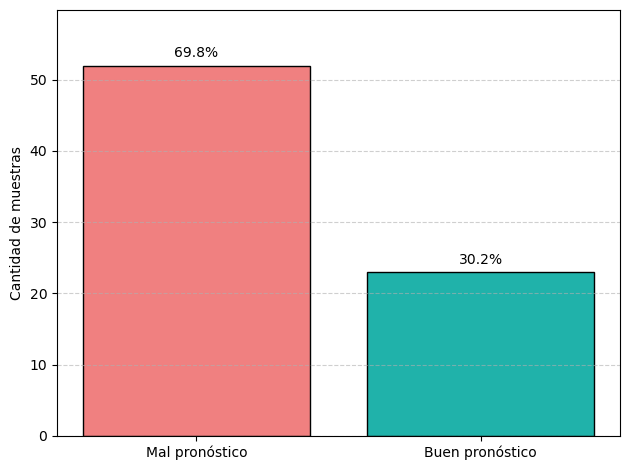
\includegraphics[width=0.25\linewidth]{img/class_distr_eval.png}
    }
    \caption{Distribución de clases en los distintos conjuntos de datos}
    \label{fig:distr}
\end{figure}


En \ref{fig:classDistrCompl} podemos ver como el dataset completo tiene un 69,8\% de datos etiquetados por mal pronostico y un 30,2\% de buen pronostico, y en \ref{fig:distr1} y \ref{fig:distr2} vemos como el conjunto de entrenamiento y evaluación 
mantienen la misma proporción de clases que el dataset completo.


\section*{Árboles de decisión}

Este ejercicio consistía de la construcción de modelos de tipo árbol de decisión, y luego realizar una estimación de performance de estos.
El primer objetivo realizado fue construir un arbol con altura máxima 3 con sus parametros en default. Luego, realizamos un K-fold cross validation sobre este utilizando distintas métricas (Accuracy, AUC-PRC y AUC-ROC). La idea era calcular las métricas utilizando tanto el promedio de los resultados de cada fold, como también el score global para los folds de validación, utilizando siempre los mismos folds.

\begin{table}[h!]
\centering
\resizebox{\textwidth}{!}{
\begin{tabular}{lcccccc}
\hline
    & \textbf{Acc. (Val)} & \textbf{Acc. (Train)} & \textbf{AUC ROC (Val)} & \textbf{AUC ROC (Train)} & \textbf{AUC PRC (Val)} & \textbf{AUC PRC (Train)} \\
\hline
0 & 0.588235 & 0.823529 & 0.520333 & 0.846545 & 0.311156 & 0.650633 \\
1 & 0.670588 & 0.802941 & 0.636533 & 0.822029 & 0.337906 & 0.673870 \\
2 & 0.647059 & 0.826471 & 0.584827 & 0.839358 & 0.445933 & 0.638929 \\
3 & 0.670588 & 0.820588 & 0.649425 & 0.840051 & 0.418101 & 0.675693 \\
4 & 0.658824 & 0.794118 & 0.664276 & 0.836437 & 0.375702 & 0.681502 \\
\hline
\textbf{Promedios} & 0.647059 & 0.813529 & 0.611079 & 0.836884 & 0.377759 & 0.664125 \\
\textbf{Global} & 0.647059 & -- & 0.507207 & -- & 0.305654 & -- \\
\hline
\end{tabular}
}
\caption*{Resultados de validación cruzada}
\label{tab:resultados_cv}
\end{table}

Analicemos los resultados para cada métrica, considerando el modelo usado, la cantidad de atributos de nuestras instancias, y el desbalance de clases que tienen los datos.
\begin{itemize}
    \item \textbf{Accuracy} (Acc.): notemos que su valor en datos de validación es $\approx 0.65$. Pensando en que los datos de entrenamiento tienen 69,8\% de instancias de clase negativa, este resultado es peor que lo que conseguiría un clasificador que siempre predice la clase más frecuente. En función de esta métrica, se sugiere que el modelo no está aprendiendo demasiado de los datos. 
    \item \textbf{AUC-ROC}: de la misma forma, un clasificador que predice siempre la clase más frecuente tendría un AUC-ROC de $0.50$, y nuestro modelo lo supera apenas con $\approx 0.6110$ con el promedio de sus folds, y tiene aproximadamente el mismo score en el valor global.
    \item \textbf{AUC-PRC}: tenemos un resultado análogo. En este caso, los valores absolutos son más bajos aún, y tiene sentido considerando que AUC-PRC sólo se calcula en función de Precision y Recall: estamos teniendo en cuenta sólo los valores de false positive, false negative, true positive. Como nuestros datos de entrenamiento están desbalanceados a favor de la clase negativa, que esta métrica que no tenga en cuenta los valores de true negative afecta bastante el resultado. Un clasificador que nos da siempre la clase más frecuente tendría valor  $\approx 0.30$ de AUC PRC, correspondido a nuestra proporción de 30.2\% de instancias positivas. El valor que nos dio está por debajo de ese valor en cuanto a validación, pero es un poco mayor en entrenamiento. 
     
\end{itemize}

En cada caso, vemos que los puntajes en datos de entrenamiento superan ampliamente lo que sería elecciones aleatorias o de clase más frecuente para cada métrica. La diferencia con los valores durante la validación nos sugiere sobreajuste del modelo. La causa más probable es que las instancias tienen 200 atributos y el árbol evaluado tiene como límite altura 3. Con esta limitación, al modelo le falta complejidad para capturar patrones complejos de los datos, pudiendo aprender instancias ya vistas, pero teniendo baja capacidad de generalizar a instancias nuevas.

\subsection*{Exploración de hipérparametros}	
Luego de realizar la validación cruzada, el siguiente paso fue realizar una búsqueda de hipérparametros. Para ello, volvimos a hacer un K-fold cross validation, pero esta vez con un Grid Search de los parámetros de altura máxima y el criterio de corte utilizado (Gini y Entropia). Guardamos el score conseguido con cada combinación de parámetros y chequeamos su Accuracy tanto en training como en validación. La siguiente tabla muestra los resultados obtenidos.

\begin{table}[H]
    \centering
    \begin{tabular}{cccc}
    \hline
    \textbf{Altura máxima} & \textbf{Criterio} & \textbf{Accuracy (training)} & \textbf{Accuracy (validación)} \\ \hline
    3 & Gini     & 0.813529 & 0.647059 \\ \hline
    5 & Gini     & 0.921176 & 0.670588 \\ \hline
    Infinito & Gini     & 1.000000 & 0.663529 \\ \hline
    3 & Entropía & 0.768235 & 0.665882 \\ \hline
    5 & Entropía & 0.892941 & 0.656471 \\ \hline
    Infinito & Entropía & 1.000000 & 0.647059 \\ \hline
    \end{tabular}
    \caption*{Resultados de accuracy para diferentes alturas y criterios.}
    \label{tab:accuracy_arboles}
\end{table}
    
Con ambos criterios se puede ver que al no limitar la altura máxima del árbol (o sea, altura máxima = Infinito),
el accuracy de entrenamiento es 1, lo cual indica que el modelo ajusta a perfectamente a los datos de entrenamiento y sabe clasificar instancias ya vistas. Sin embargo, en todos los casos el accuracy de validación es menor que lo que conseguiría un modelo que predice la clase más frecuente (siendo que tenemos 68\% de instancias de clase negativa), y en todos los casos se tiene una brecha amplia con el score de entrenamiento. Esto nos da a entender que los modelos planteados están sobreajustados y no pueden generalizar a partir de lo que aprendieron en entrenamiento. 

En el caso de usar Gini, al aumentar la altura máxima del árbol de 3 a 5, el accuracy de validación mejora. Sin embargo, también aumentan el accuracy de entrenamiento y la brecha entre los dos puntajes. En el caso de entropía, con el aumento de altura entre 3 y 5, se ve incluso una disminución en el accuracy de validación, sugiriendo una generalización incluso peor al separar los datos bajo este criterio con un nivel más.

\section*{Comparación de algoritmos}

En esta sección, nos concentramos en la implementación de diferentes algoritmos de clasificación, para luego testear la performance de cada uno de ellos.
En particular, utilizamos los algoritmos de \textit{K-vecinos Más Cercanos} (KNN), \textit{Support Vector Machine} (SVM) y \textit{Árboles de Decisión}. 
A su vez, en cada uno de estos algoritmos, realizamos una búsqueda de hiperparámetros, utilizando Randomized Search, para encontrar la mejor combinación
posible.

\subsection*{Árboles de decisión}
Para árboles de decisión, decidimos utilizar los siguientes hiperparámetros para realizar la búsqueda:
\begin{itemize}
    \item \texttt{max\_depth}: Profundidad máxima del árbol. Probamos un rango de alturas entre 1 y 25, teniendo en cuenta que la altura del árbol balanceado sería $log_2(425) = 9$.
    \item\texttt{Criterion}: los vistos en clase, \textit{Gini} y \textit{Entropy}, y \textit{log loss}.

    \item \texttt{min\_samples\_split}: Número mínimo de muestras requeridas para dividir un nodo.
    
    \item \texttt{min\_samples\_leaf}: Número mínimo de muestras requeridas para estar en una hoja.
    
    \item \texttt{max\_features}: Número máximo de características a considerar al buscar la mejor división. En este caso, probamos con un máximo de 1, 3, sqrt y log$_2$, e ilimitado.
\end{itemize}

Las 6 mejores configuraciones obtenidas respecto a la métrica \textit{AUC-ROC} fueron las siguientes:

\begin{table}[H]
    \centering
    \begin{tabular}{|l|c|c|c|c|c|c|}
    \hline
    \textbf{Modelo} & \textbf{Min Samples Split} & \textbf{Min Samples Leaf} & \textbf{Max Features} & \textbf{Max Depth} & \textbf{Criterion} & \textbf{AUC-ROC} \\
    \hline
    \rowcolor{yellow!30}
    Árbol 1 & 10 & 4 & none & 6 & entropy & 0.646 \\
    Árbol 2 & 5 & 4 & sqrt & 9 & log\_loss & 0.643 \\
    Árbol 3 & 5 & 2 & none & 12 & entropy & 0.637 \\
    Árbol 4 & 2 & 2 & none & 12 & log\_loss & 0.634 \\
    Árbol 5 & 10 & 2 & none & 24 & log\_loss & 0.634 \\
    Árbol 6 & 5 & 2 & none & 23 & entropy & 0.632 \\
    \hline
    \end{tabular}
    \caption*{Mejores modelos de la búsqueda - Árboles de decisión}
    \label{tab:hiperparametros-arboles-tabla}
\end{table}

Los resultados están todos por debajo de 0.7. Esto puede ser debido a que
el árbol de decisión no está logrando captar el patrón de los datos, por lo que no logra generalizar correctamente y
ofrecer un buen resultado. La distribución de los datos puede influir fuertemente en esto, lo cual podría cambiar significativamente
si las etiquetas se distrubuyesen de manera distinta. Sin embargo, con el dataset que tenemos, el árbol de decisión no parecería ser ideal.
\subsection*{K-vecinos más cercanos}

El siguiente algoritmo en el que realizamos una búsqueda de hiperparametros fue KNN. En este algoritmo no buscámos sobre
muchos hiperparámetros distintos, sino que buscamos solo entre 3, que son los que consideramos más relevantes:
\begin{itemize}
    \item \texttt{n\_neighbors}: Número de vecinos a considerar. Probamos con un rango de 1 a 30,
    \item \texttt{p}: El tipo de distancia a utilizar. En este caso, probamos con \textit{euclidiana} y \textit{manhattan}.
    \item \texttt{algorithm}: consideramos \textit{ball tree}, \textit{kd tree} y \textit{brute}. Además, tambien probamos con el parámetro \textit{auto}, que selecciona el mejor algoritmo a utilizar dependiendo de los datos.
\end{itemize}

Veamos ahora los mejores resultados obtenidos con el Randomized Search. En este caso, nos quedamos nuevamente con las mejores 
6 combinaciones obtenidas respecto a la métrica \textit{AUC-ROC}. Estas son las siguientes:

\begin{table}[H]
    \centering
    \begin{tabular}{|l|c|c|c|c|c|c|}
    \hline
    \textbf{Modelo} & \textbf{N Neighbors} & \textbf{Distancia (p)} & \textbf{Algorithm} & \textbf{AUC-ROC} \\
    \hline
    \rowcolor{yellow!30}
    KNN 1 & 20 & Manhattan & brute & 0.865 \\
    KNN 2 & 11 & Manhattan & kd\_tree & 0.865 \\
    KNN 3 & 15 & Manhattan & kd\_tree & 0.859 \\
    KNN 4 & 13 & Manhattan & brute & 0.859 \\
    KNN 5 & 17 & Manhattan & ball\_tree & 0.856 \\
    KNN 6 & 27 & Manhattan & ball\_tree & 0.853 \\
    \hline
    \end{tabular}
    \caption*{Mejores modelos de la búsqueda - K-vecinos más cercanos}
    \label{tab:hiperparametros-knn-tabla}
\end{table}

En este caso podemos ver una mejora enorme en los resultados obtenidos respecto a los árboles de decisión. Ya con valores
superiores a 0.8, podemos decir que el modelo se comporta bastante bien, y representaría una mejor elección de algoritmo que
los árboles de decisión para este dataset. 

Puede observarse también en la tabla que conseguimos el mismo resultado con otra combinación de hiperparámetros, y que, 
además, con otras configuraciones, los otros resultados obtenidos son bastante similares y se acercan mucho al valor máximo
conseguido.

\subsubsection*{SVM}

El último algoritmo que probamos fue SVM. Realizamos una búsqueda sobre los siguientes hiperparámetros:
\begin{itemize}
    \item \texttt{C}: Parámetro de regularización. Probamos con los valores 0.1, 1, 10 y 100.
    \item \texttt{kernel}: Tipo de kernel a utilizar. En este caso, probamos con \textit{linear}, \textit{poly}, \texttt{rbf} y \textit{sigmoid}.
    \item \texttt{gamma}: El coeficiente utilizado para el kernel. Los posibles parámetros fueron \textit{scale} y \texttt{auto} 
\end{itemize}

Veamos a continuación los resultados de la búsqueda de hiperparámetros:

\begin{table}[H]
    \centering
    \begin{tabular}{|l|c|c|c|c|c|c|}
    \hline
    \textbf{Modelo} & \textbf{C} & \textbf{Kernel} & \textbf{Gamma} & \textbf{AUC-ROC} \\
    \hline
    \rowcolor{yellow!30}
    SVM 1 & 100 & rbf & scale & 0.918 \\
    SVM 2 & 10 & rbf & scale & 0.918 \\
    SVM 3 & 0.1 & rbf & scale & 0.869 \\
    SVM 4 & 0.1 & poly & auto & 0.821 \\
    SVM 5 & 10 & poly & auto & 0.821 \\
    SVM 6 & 1 & poly & auto & 0.821 \\
    \hline
    \end{tabular}
    \caption*{Mejores modelos de la búsqueda - K-vecinos más cercanos}
    \label{tab:hiperparametros-knn-tabla}
\end{table}

Observemos que hay un resultado muy interesante: al usar los hiperparametros \textit{kernel = poly} y \textit{gamma = auto},
el modelo logra un AUC-ROC de 0.832 sin importar que \textit{C} varíe entre 0.1 y 100. Es decir, usando esos hiperparámetros
no afectó cambiar el parámetro de regularización, y funcionó igual independientemente de si lo variamos.
Por otro lado, ocurrió algo similar utilizando \textit{kernel = rbf} y \textit{gamma = scale}, donde tuvimos un resultado de 
0.918 usando \textit{C = 100} y \textit{C = 10}, y siendo este el valor más alto obtenido utilizando este algoritmo. Sin embargo,
si se observa una diferencia cuando \textit{C = 0.1}, ya que el AUC-ROC baja a 0.869.

\subsection*{Comparación final}

Para continuar aun mas con la comparación de algoritmos introdujimos también un modelo de \textit{Linear Discriminant Analisys (LDA)} y uno de \textit{Naive Bayes}.
Sin embargo, no realizamos una búsqueda de hiperparámetros para ellos, sino que los dejamos en default.

Finalmente, realizamos una comparación entre los algoritmos implementados utilizando la mejor configuración de hiperparámetros
para cada caso (es decir, la que consiguió el mejor AUC-ROC en cada algoritmo), que se puede visualizar en la figura \ref{fig:comparacion-modelos}. Además, comparamos los valores conseguidos
con los de LDA y Naive Bayes. 

Notemos que los árboles de decisión tuvieron la peor performance para el dataset utilizado. LDA y Naive Bayes ofrecieron una
mejora considerable junto con KNN, pero el mejor resultado fue el de SVM, que logró un AUC-ROC de 0.918. Claramente SVM fue el 
algoritmo que mejor logra entender el dataset, y logra generalizar de muy buena manera para nuevas instancias.

\begin{figure}[h]
    \centering
    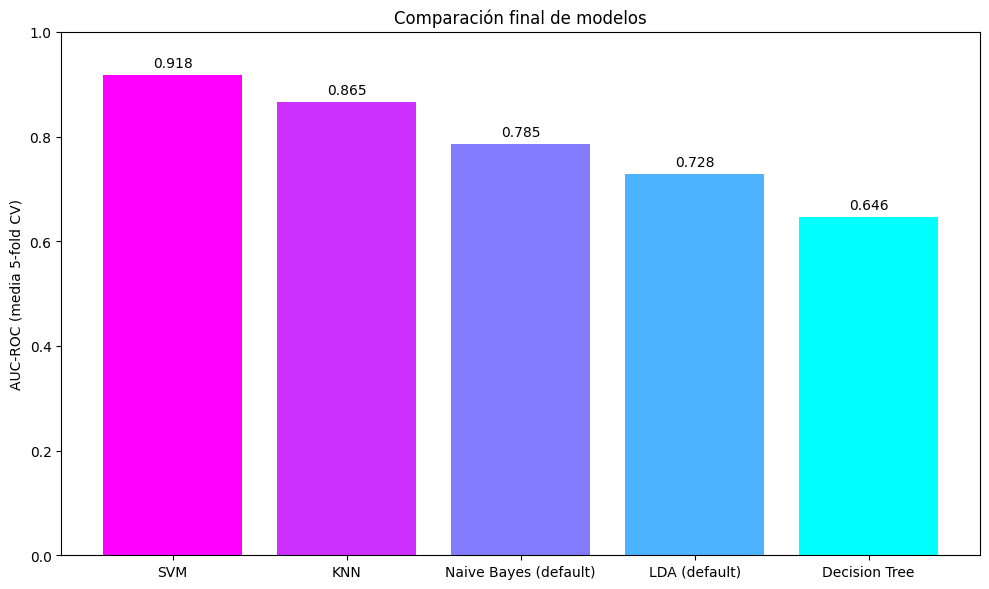
\includegraphics[width=0.60\linewidth]{img/comparacion-modelos.png}
    \caption*{Comparación final de mejores modelos}
    \label{fig:comparacion-modelos} 
\end{figure}


Observemos también que los modelos que consiguieron mejor performance fueron aquellos que se comportan mejor con una distribución normal de los datos, como es el caso de SVM utilizando el kernel radial, y modelos que asumen normalidad, como LDA y Naive Bayes. Además, KNN, que se basa en distancias, tuvo un rendimiento muy bueno, 
superior al de LDA y Naive Bayes, pero no tanto como el de SVM.

\section*{Diagnóstico de sesgo y varianza}
En pos de entender cómo se comportan el sesgo y la varianza en nuestros modelos, realizamos mediciones para
construir curvas de complejidad y aprendizaje para tres de nuestros mejores modelos: KNN, SVM y Árboles de Decisión.

\subsection*{Curvas de Complejidad}
Usando nuestros mejores modelos obtenidos durante la exploración de hiperparámetros, graficamos el desarrollo del error
a partir de cambiar ciertos hiperparámetros de cada modelo. Observemos a continuación cómo quedaron los gráficos:

\begin{figure}[H]
    \centering

    \subfloat[\centering Curva de complejidad para Árboles \label{fig:comp1}]{
        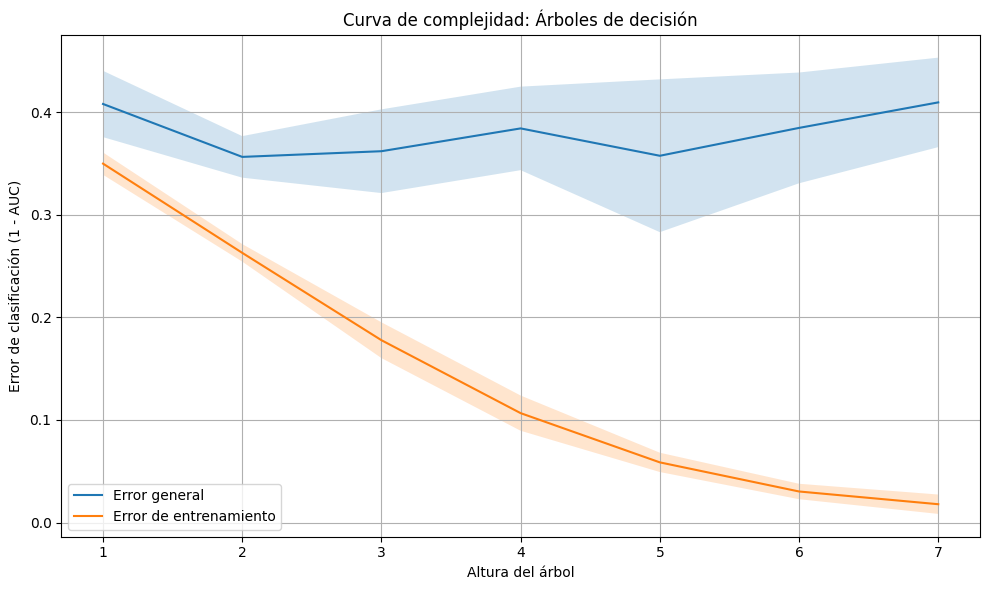
\includegraphics[width=0.5\linewidth]{img/complejidad_arbol.png}
    }
    \subfloat[\centering Curva de complejidad para SVM \label{fig:comp3}]{
        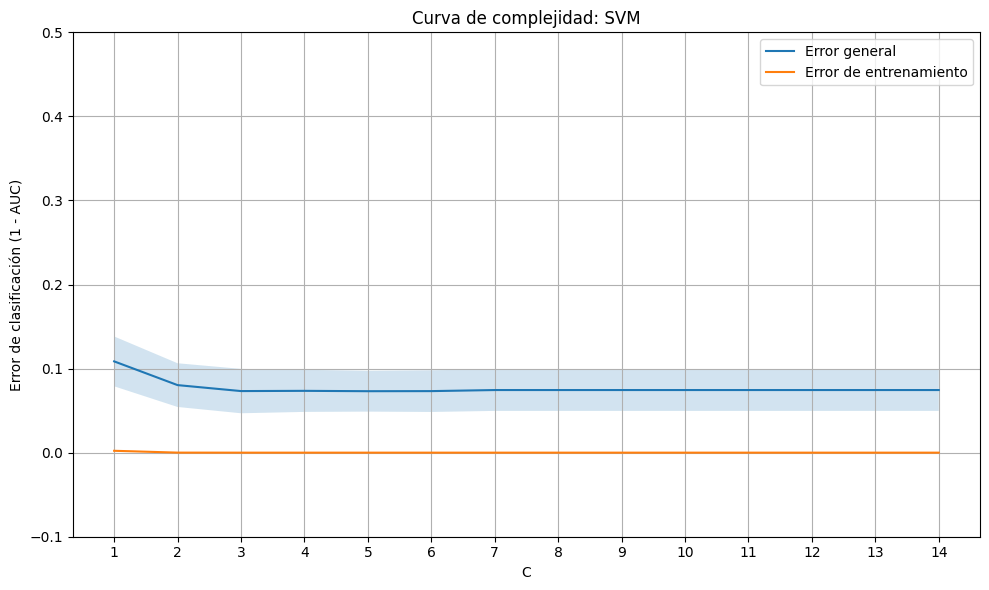
\includegraphics[width=0.5\linewidth]{img/complejidad_svm.png}
    }
 
    \vspace{0.1cm}

    \subfloat[\centering Curva de complejidad para KNN \label{fig:comp2}]{
        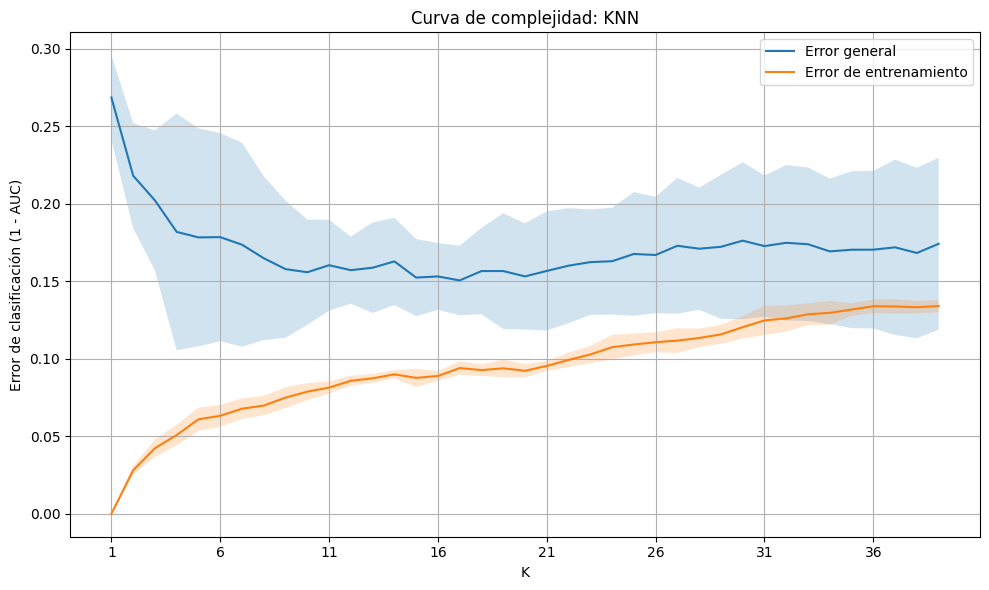
\includegraphics[width=0.5\linewidth]{img/complejidad_knn.png}
    }
    \label{fig:distr}
\end{figure}

Las curvas muestran el error, el cual computamos como 1 - \textit{AUC-ROC} en funcion del hiperparámetro explorado, donde 
el error general es a partir de la predicción del fold que no usó para entrenar, y el error de entrenamiento surge de predecir los mismos datos
utilizados para entrenar el modelo.

En \ref{fig:comp1}, podemos ver que para el \textbf{Decision Tree} calculamos el error con distintos valores de la altura desde 1 a 10, ya que explorar valores mas altos no aporta
más ganancia en este dataset.

A medida que aumenta la altura del árbol, el sesgo disminuye significativamente, dejando el error de entrenamiento en 0. Sin 
embargo, el error general no baja a medida que aumenta la altura del árbol, aumentndo la varianza y mostrando que el modelo está 
overfitteando. Por otro lado, en las alturas más bajas del árbol se ve un error de entrenamiento muy alto, mostrando que, en estas
circunstancias, el modelo subajusta. La altura óptima para este modelo sería entre 2 y 5, ya que hay un buen \textit{trade-off} entre
el sesgo y la varianza.

Observando \ref{fig:comp3}, podemos notar que el modelo de \textbf{Support Vector Machines} comienza teniendo un error general alto y un error de entrenamiento muy bajo,
indicando alto sesgo. Sin embargo, al agrandar \texttt{C}, el error general baja entre hasta \texttt{C} = 1 y \texttt{C} = 3, y luego se mantiene constante; mientras que el error
de entrenamiento se mantiene bajo, por lo que el sesgo baja significativamente, y la varianza se mantiene en valores bajos.
Esto indica que este modelo SVM ya tiene suficiente flexibilidad para separar bien las clases y añadir capacidad extra (agrandando el valor de \texttt{C}) no empeora la generalización.

En cuanto a \textbf{K-Nearest Neighbors}, en \ref{fig:comp2} se observa un comportamiento contrario al de los árboles. Valores bajos de \texttt{K} llevan a modelos que sobreajustan. Al subir este hiperparámetro, 
el modelo comienza a subajustar. Con \texttt{K} bajos, el modelo se acopla perfectamente a los datos de entrenamiento,
produciendo bajo sesgo y alta varianza. Con \texttt{K} entre 7 y 15, se observan los valores óptimos de  \textit{trade-off} entre sesgo y varianza,
y, al llegar a los valores más altos de \texttt{K}, se reduce notablemente la varianza, con una suba considerable de el sesgo.


\subsection*{Curvas de Aprendizaje}
Para los mismos modelos, también graficamos curvas de aprendizaje. Hicimos uso de la función de de la biblioteca scikitlearn llamada \texttt{learning\_curve}. Como parámetro de cuántas instancias contemplar en el conjunto de entrenamiento, usamos un array de 5 valores equitativamente espaciados entre 0.1 y 1.0, que representa la proporción de instancias utilizadas en cada ejecución. Al hacer 5-fold cross validation para armar las curvas, terminamos entrenando con 34, 110, 187, 263 y 340 instancias a la vez.

\begin{figure}[H]
    \centering

    \subfloat[\centering Curva de aprendizaje para árboles de decisión \label{fig:apr1}]{
        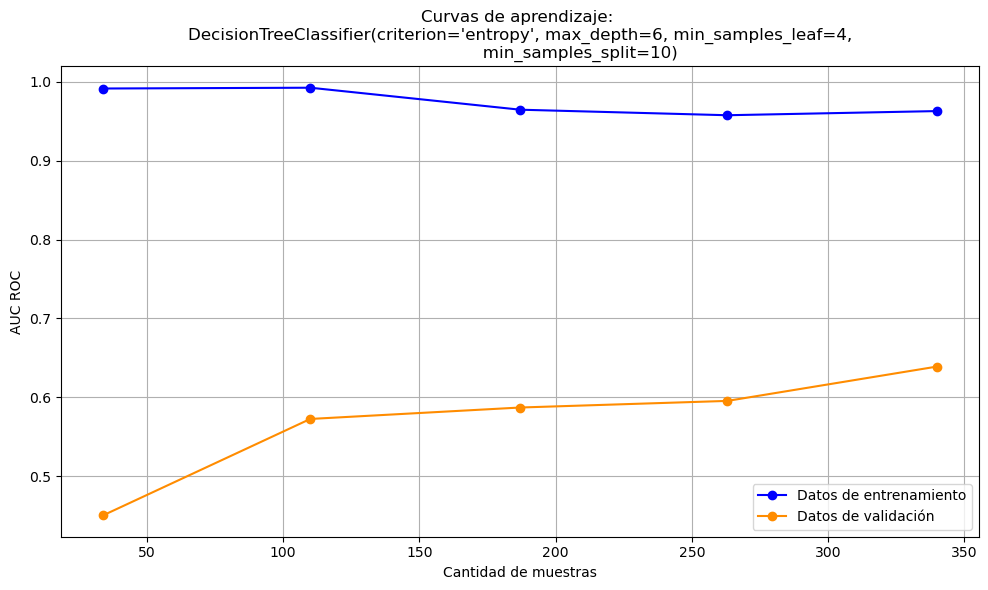
\includegraphics[width=0.45\linewidth]{img/aprendizaje_arbol.png}
    }
    \subfloat[\centering Curva de complejidad para SVM \label{fig:apr3}]{
        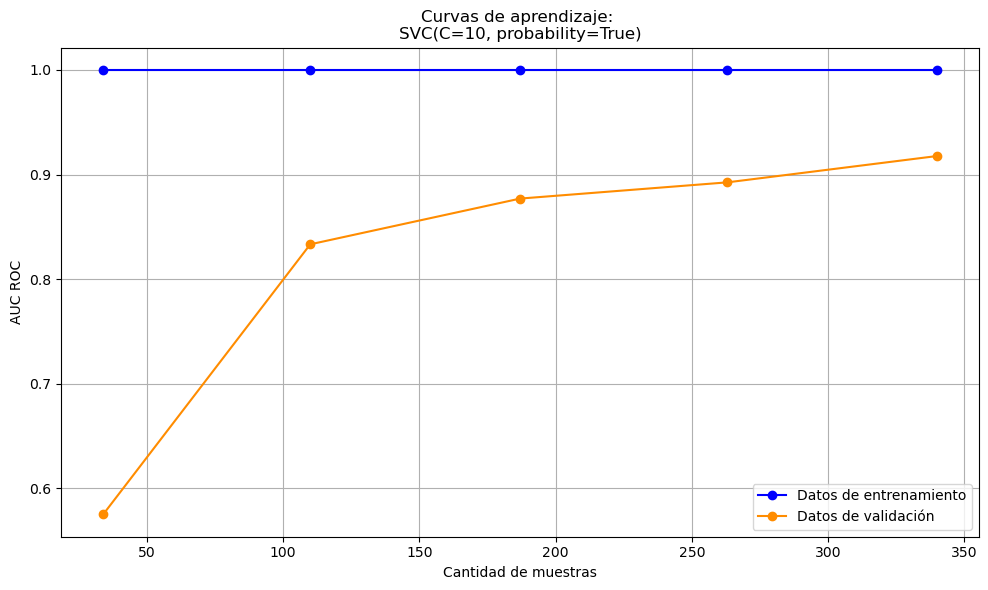
\includegraphics[width=0.45\linewidth]{img/aprendizaje_svm.png}
    }

    \vspace{0.3cm}

    \subfloat[\centering Curva de aprendizaje para KNN \label{fig:apr2}]{
        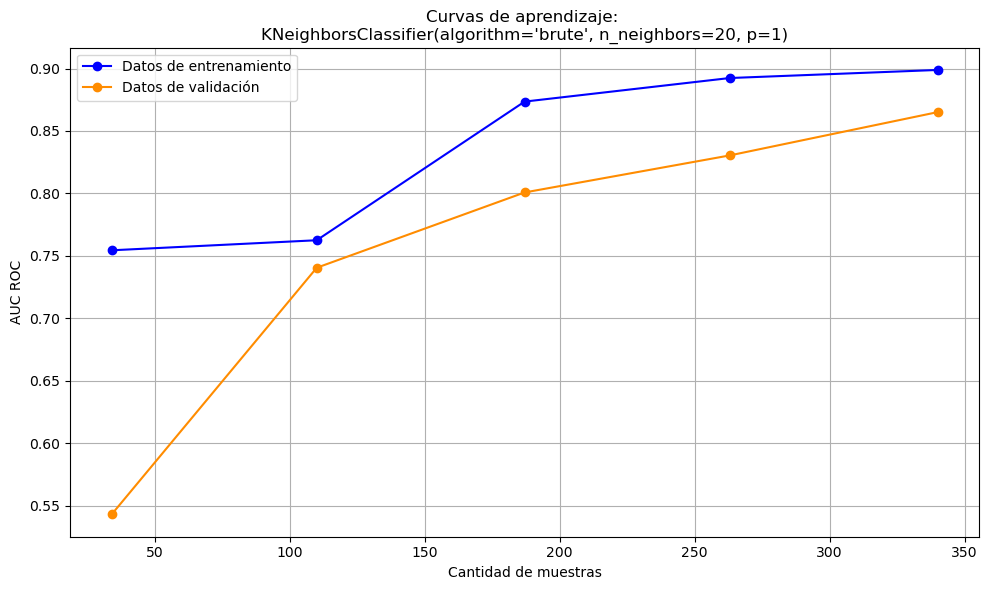
\includegraphics[width=0.45\linewidth]{img/aprendizaje_knn.png}
    }
    \subfloat[\centering Curva de aprendizaje para LDA \label{fig:apr4}]{
        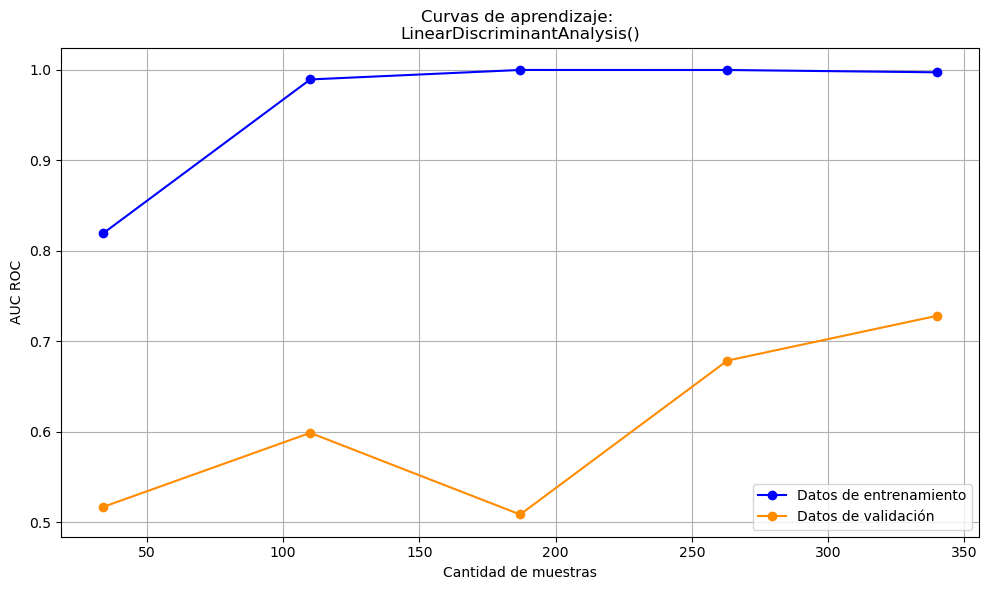
\includegraphics[width=0.45\linewidth]{img/aprendizaje_lda.png}
    }

    \caption{Curvas de complejidad para distintos modelos}
    \label{fig:distr}
\end{figure}

Para \textbf{árboles de decisión}, en la figura \ref{fig:apr1}, con las primeras proporciones de instancias de entrenamiento (34 y 110 instancias), el modelo parece estar sobreajustando. Vemos que en entrenamiento tiene un AUC-ROC tendiente a 1, pero en los datos de evaluación el AUC-ROC está por debajo o apenas supera AUC-ROC de 0.5 que tendría un clasificador dummy. Pero a medida que incrementa la proporción de datos utilizados para entrenar, también incrementa el AUC-ROC de validación y disminuye el de entrenamiento, achicando la brecha entre estos. Podemos asumir que con una proporción baja de datos de entrenamiento el modelo no lograba captar patrones subyacentes a los datos, aprendiendo características que le permitían ajustar a los datos que conocía pero que no eran representativos del dataset en general.

En cuanto a \textbf{Support Vector Machines}, en la figura \ref{fig:apr3} se puede ver que la performance en evaluación medida con AUC-ROC sube muchísimo al aumentar la cantidad de muestras, principalmente entre 1 y 110. Luego de las 100 muestras, el modelo sigue mostrando mejoras en su comportamiento, pero con incrementos más suaves. Sin embargo, más allá de que el puntaje en evaluación mejora, la performance sobre los datos de entrenamiento se mantiene en 1 sin importar la cantidad de muestras que se usen para entrenar, lo cuál puede indicar un sobreajuste cuando se cuenta con bajas cantidades de datos.

Para \textbf{K-Nearest Neighbors}, podemos interpretar la figura \ref{fig:apr2} en base al hiperparámetro de \texttt{n\_neighbors}, que en nuestro mejor modelo es 20. Esto es un número bastante elevado en comparación a con cuántas instancias entrenamos en las primeras iteraciones. No es sorpresivo que con 20 vecinos, usando 34 instancias, el AUC-ROC de entrenamiento sea relativamente bajo y el de evaluación ($\approx 0.55$) sea similar al AUC-ROC del clasificador que predice la clase más frecuente; ya que estamos seleccionando \texttt{n\_neighbors} $\approx$ cantidad de instancias. Al incrementar la cantidad de instancias vistas, podemos ver que todos los puntajes AUC-ROC aumentan proporcionalmente, tanto los de entrenamiento como los de validación.


Y por último, con \textbf{Linear Discriminant Analysis}, en la figura \ref{fig:apr4} la performance en entrenamiento aumenta a medida que subimos la cantidad de muestras hasta 187, y luego se mantiene constante. Sin embargo, cuando observamos el AUC-ROC con datos de validación, el gráfico presenta más variaciones, alcanzando el mínimo cuando se entrena con 187 muestras. Esto puede sugerir que en esa iteración el modelo sobreajusta sobre los datos de entrenamiento, y no logra generalizar correctamente para nuevas instancias. Podría estar relacionado a qué instancias en particular fueron agregadas a la muestra en esa iteración. Sería posible que ese conjunto de 187 muestras no sea representativo de la distribución del conjunto de los datos, impidiendo aprender características útiles para generalizar. Luego de alcanzar el mínimo, si seguimos aumentando la cantidad de instancias la performance en validación sí mejora significativamente.


\subsection*{Exploración de Random Forest}
Para este experimento, construimos un modelo Random Forest con 200 árboles. La idea fue explorar el hiperparámetro \texttt{max\_features}, que limita cuántos atributos se pueden considerar cada vez que se busca el mejor corte para el árbol. Los valores considerados fueron  1, $log_2(\#atributos)$, 10, $sqrt(\#atributos)$, 50, 100, 200 (es decir, $\#atributos$).
 \begin{figure}[H]
    \centering

    \subfloat[\centering Curvas de complejidad variando el hiperparámetro \texttt{max\_features} \label{fig:rf1}]{
        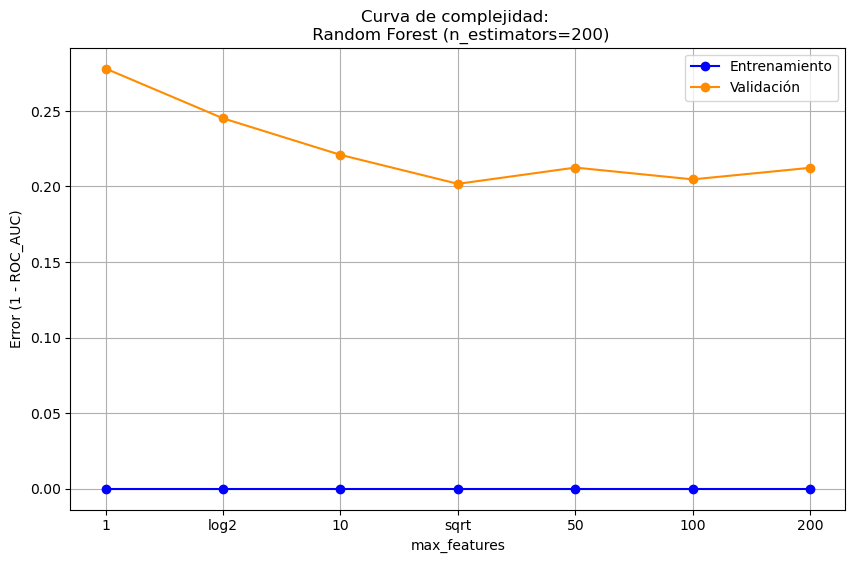
\includegraphics[width=0.45\linewidth]{img/rf1.png}
    }
    \subfloat[\centering Curvas de aprendizaje utilizando \texttt{max\_features} = $sqrt(\#atributos)$ \label{fig:rf2}]{
        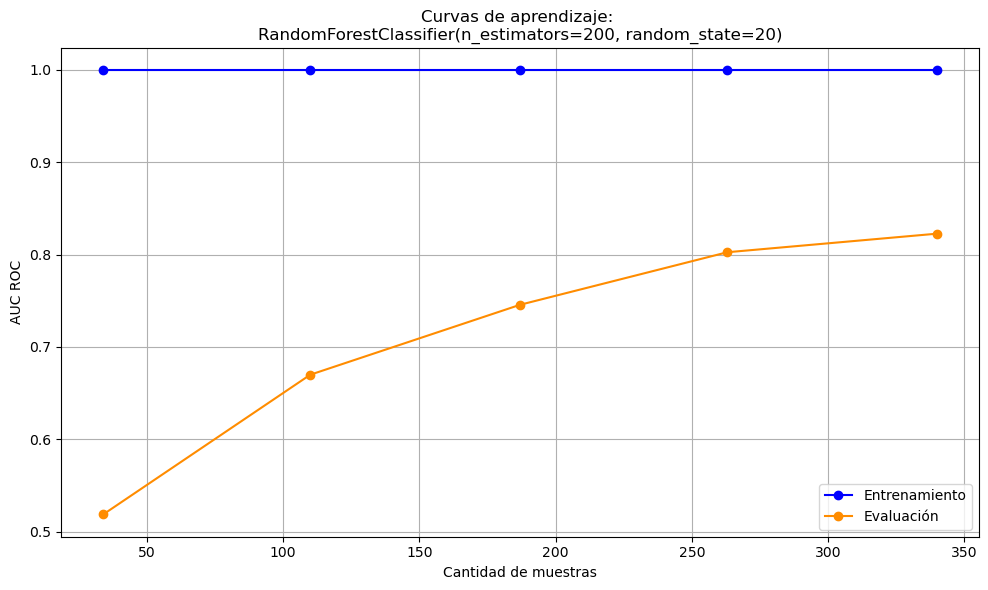
\includegraphics[width=0.45\linewidth]{img/rf2.png}
    }
    \caption{Resultados de experimentos con Random Forest}
    \label{fig:distr}
\end{figure}

En la figura \ref{fig:rf1} generamos curvas de complejidad para cada uno de los modelos resultantes, en base a estos valores de \texttt{max\_features}. Con los datos de entrenamiento, cualquier cantidad de atributos genera un árbol que ajusta perfectamente. La diferencia se ve en los datos no vistos en entrenamiento. Podemos observar que el error en validación es mínimo utilizando $sqrt(\#atributos) \approx 14$. También que se llega al mayor error con los valores más bajos: con 1, $log_2 \approx 8$ y 10. Es decir, elegiríamos no limitar más que $sqrt(\#atributos)$ la cantidad de atributos máxima a contemplar en los cortes. Contemplar menos atributos parece limitar la capacidad de generalización del modelo.

Utilizando el mínimo valor observado, \texttt{max\_features} $= sqrt(\#atributos)$, graficamos también una curva de aprendizaje, que se puede visualizar en la figura \ref{fig:rf2}. Podemos ver una evolución considerable en la performance con datos de validación. A medida que aumentamos la cantidad de datos, también sube la performance, llegando hasta AUC-ROC de $\approx  0.83$. Sin embargo, más allá de que la curva sube, se observa que el aumento de performance no es constante, y tiende a estancarse, por lo que agregar más datos no debería presentar un aumento significativo. Por otro lado, la performance en entrenamiento se mantiene constante sin importar la cantidad de muestras utilizadas, presentando un AUC-ROC de 1 tomando tanto la mínima cantidad de muestras como la máxima. A partir de esto, podríamos estar ante un sobreajuste cuando tenemos baja cantidad de instancias, y, a medida que aumentan, el modelo comienza a generalizar mejor.


\section*{Conclusiones}

Finalmente, con todos los analisis realizados, hicimos la validación final usando los datos de test 
que nos separamos al principio. Para esta evaluación probamos con los mejores modelos 
de \textbf{RandomForest}, \textbf{K-NN} y \textbf{SVM}, los resultados fueron los siguientes:
\begin{table}[H]
    \centering
    \begin{tabular}{l|cc}
        \hline
        \textbf{Modelo} & \textbf{AUC-ROC} & \textbf{Accuracy} \\ \hline
        RandomForest & 0.8039 & 0.7067 \\ \hline
        KNN & 0.8633 & 0.7867 \\ \hline
        SVM & 0.9204 & 0.88 \\ \hline
    \end{tabular}
    \caption*{Resultados finales con datos de test}
    \label{tab:resultados}
\end{table}

Los mejores resultados se obtienen usando \textbf{SVM}, así que el \textit{held\_out} final lo
realizamos con este modelo.

Notemos que el \textit{AUC-ROC} de test en SVM nos dio ligeramente más alto que en el Cross Validation.
Nuestra hipótesis de porqué está ocurriendo esto es que el modelo aprendió muy bien a separar las clases,
y dado que los datos de test son pocos, ya por cuestiones de azar, el modelo logró generalizar mejor en test.
La distribución de clases es igual en train y test, por lo que se comporta como esperamos.

El hecho de que los mejores modelos sean los que encuentran patrones no lineales
en los datos, como \textbf{SVM} y \textbf{KNN}, nos indica que el dataset tiene una separación no lineal entre las clases.
En \textbf{SVM} el kernel radial es el que mejor clasifica, esto nos indica que los datos pueden estar
distribuidos de una forma similar a una normal.
Esto tambien aplica en \textbf{LDA} y \textbf{Naive Bayes} que asumen esta condición sobre los datos.

\subsection*{Oversampling}
Nos encontramos frente a un dataset desbalanceado,
es muy posible que el modelo aprenda a predecir la clase mayoritaria y no generalice bien.
Para evitar esto, podemos aplicar oversampling a la clase minoritaria.
Inyectando datos sintéticos a la clase minoritaria para que haya una distribución equitativa de clases en el entrenamineto.

Por el momento reconocemos este problema y lo dejamos como tarea a futuro, en este trabajo nos centramos en entender como distintos modelos
y configuraciones especificas varian la performance y predicciones esperadas.

%\part*{Referencias}
%\bibliographystyle{plain}
%\bibliography{refs}

\end{document}
